\chapter{Objektivní metody hodnocení kvality zvuku}
\label{chap:objectiveMetods}

\epigraph{\hfill\textit{Práce je to, co nikdo nechce dělat.}}{Tomáš Garrigue Masaryk}

Jak už je naznačeno v úvodu, objektivní algoritmy slouží jako alternativa k subjektivním poslechovým testům. Jde o způsob jakým obejít mnohdy náročné testování s velkým počtem posluchačů a tím ušetřit nemalé množství materiálních i časových prostředků.

Snaha o objektivní hodnocení za použití výpočetních metod se dá vysledovat až k počátkům devadesátých let. Existuje několik metod a pohledů na tuto problematiku, nicméně všechny v jádru sdílí obdobný přístup. Konkrétně snahu o modelování lidské sluchové cesty, dále přepočet na vnitřní koeficienty reprezentující nervové vzruchy a v závěru jejich matematické zpracování, často označované jako kognitivní analýza. Výsledkem bývá numerická hodnota odpovídající umístění na hodnotící škále, stejně jako tomu je při subjektivním testování.

V čem se metody liší je jejich zaměření a oblast použití. Telekomunikační sekce ITU-T, která standardizuje systémy jejichž cílem je přenést lidský hlas, se zabývá algoritmy, které sledují převážně srozumitelnost. Naproti tomu hodnocení v systémech definovaných radiokomunikační sekcí ITU-R se soustředí spíše na věrohodnost reprodukce originálního signálu v audiovizuálních systémech.

Dále by se metody daly rozdělit podle toho, zda pro svou funkci vyžadují referenci v plné kvalitě či nikoliv na tzv. \uv{Intruzivní} a \uv{Neintruzivní}. Vyhodnocování kvality řeči bývá častěji řešeno neintruzivně, jelikož algoritmy porovnávají testovaný materiál s vnitřními modely řeči. Hudba, která je zvukově \uv{rozmanitější} většinou vyžaduje přístup intruzivní.

\section{Metody užívané v telekomunikační technice}

I přes to že se tato práce nezabývá telekomunikační problematikou, je dobré zmínit jaké metody objektivního hodnocení kvality poslechu mluveného slova existují. Ať už proto, že do jisté míry sdílí vnitřní filozofii s těmi z oblasti multimediální techniky, tak proto že vývoj některých algoritmů pro hodnocení kvality hudebních nahrávek vzešel právě z této oblasti. 

%\subsection{Algoritmy definované Mezinárodní telekomunikační unií}
%\begin{itemize}
%    \item PSQM, PESQ a POLQA
\subsection{PSQM, PESQ a POLQA}    
    Jsou tři po sobě jdoucí standardy popisují intruzivní algoritmy určené k hodnocení řeči v telekomunikacích. Společně s evolucí telekomunikačního řetězce se vyvíjely i systémy objektivního hodnocení, nicméně všechny tři staví na modelování sluchové cesty a následné kognitivní analýze.
    
    Nejstarší PSQM \textit{Perceptual Speech Quality Measure} popsaný v ITU-T P.861 \cite{itut:861} v roce 1996 se soustředí na oblast telekomunikačního pásma 300 Hz - 3,4 kHz. Signály převádí do frekvenční oblasti, kde pomocí filtrů reprezentujících bazilární membránu vytvoří aproximaci zvuku, který vnímá účastník telefonního rozhovoru. Následovným porovnáváním signálů jsou určeny tři parametry:
    \begin{itemize}
        \item Časově-frekvenční zvlnění (\textit{Time-Frequency Warping})
        \item Frekvenční zvlnění (\textit{Frequency Warping})
        \item Úrovňové zvlnění (\textit{Intensity Warping})
    \end{itemize}
    Jejich váhovaným rozdílem je vypočten parametr označovaný jako $QD$ (\textit{Quality Degradation}), který je mapován na škálu $MOS$ (\textit{Mean Opinion Score}), která se používá jako výstup subjektivních testů.
    
 %   \bigskip
    
    Jako hlavní problém při hodnocení systémem PSQM se ukázalo zpožďování řeči způsobené paketovým přístupem v telefonii. Novější standard PESQ (Perceptual Evaluation of Speech Quality) dle ITU-T P.862 \cite{itut:862} principiálně popsaný obrázkem \ref{pic:pesq} tuto nevýhodu odstranil přidáním bloku \textit{Time alignment}. Ten napřed rozdělí signál na krátké úseky, v telekomunikaci zvané promluvy, korelací obálek odhadne, zda je nutná korekce a pokud ano rozdělí promluvy na rámce dlouhé 64 ms a ty pomocí výsledku korelace po vzorcích seskládá tak, aby testovaný signál odpovídal referenčnímu.
    
    \begin{figure}[h]
        \centering
        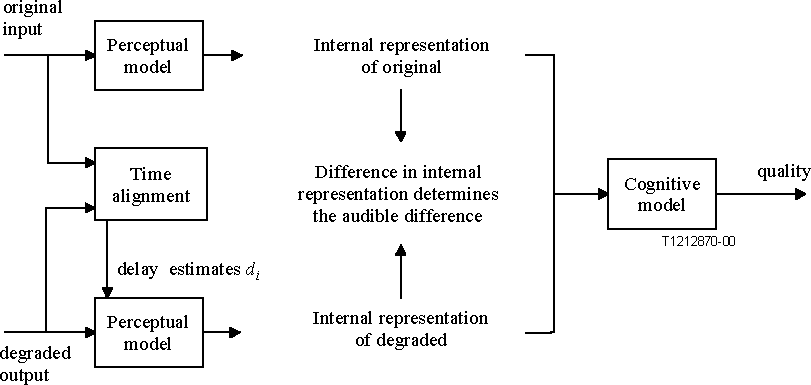
\includegraphics[width = .7\textwidth]{pic/PESQ.pdf}
        \caption{Blokové schéma algoritmu PESQ}
        \label{pic:pesq}
    \end{figure}
  
  %\bigskip
    
    Nejnovější metoda POLQA \textit{Perceptual Objective Listening Quality Assessment} dle ITU-T  P.863 z roku 2011 \cite{itut:863} řeší problematiku rozšiřovaní pásma použitého při přenosu telefonických hovorů. Definuje dva operační módy.
    \begin{itemize}
        \item Úzkopásmový: sloužící pro měření kvality v telefonním pásmu 300 Hz - 3,4 kHz. Pásmový ořez v tomto módu není považován za degradaci signálu a nemá vliv na objektivní hodnocení.
        \item Super-širokopásmový: ve kterém je šířka pásma rozšířena na 50 Hz - 14 kHz.
    \end{itemize}
    
    Princip hodnocení je podobný jako u předchozích modelů. Díky většímu výpočetnímu výkonu současných zařízení může POLQA sledovat více parametrů, a provádět složitější matematické operace při kognitivní analýze.
    
%    \item 3SQM
\subsection{3SQM}
    
    ITU–T P.563 \textit{Single Sided Speech Quality Measure} \cite{itut:536} je oproti dvěma předchozím algoritmům metodou intruzivní. Díky tomu lze využít kdekoliv v telekomunikačním řetězci a hodí se tak pro soustavné monitorování sítě. Principiální schéma je na obrázku \ref{pic:3sqm}.
    
    \begin{figure}[h]
        \centering
        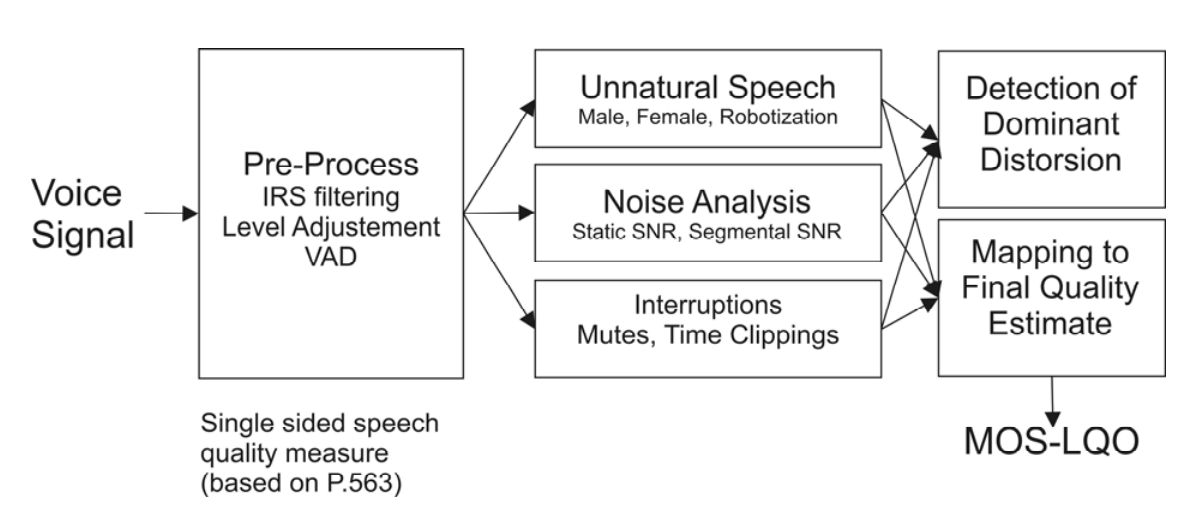
\includegraphics[width = .6\textwidth]{pic/3sqm.png}
        \caption{Blokové schéma algoritmu 3QSM}
        \label{pic:3sqm}
    \end{figure}

    Signál na vstupu prochází blokem předzpracování. Tím je normován a jsou z něj odstraněny rámce, které s řečí nesouvisí, pomocí tzv. IRS filtru (\textit{Intermediate Reference System}). Nehodí se tak pro detekci parametrů jako je zpoždění, ozvěny či poklesy hlasitosti, které mohou negativně působit na kvalitu telefonních hovorů. Samotná detekce probíhá porovnáváním úrovně obálky signálu.
    
    V signálu se poté sledují parametry jako výška hlasu, variace energie, nepřirozená periodičnost či různé druhy šumu. Na základě těchto parametrů je vytvořen pseudo-referenční signál, pomocí kterého je testovaný signál dále zpracováván intruzivním přístupem podobně jako v metodách PESQ či POLQA.
    
%\end{itemize}

\subsection{ViSQOL}
\label{subchapter:visqol}

\textit{The Virtual Speech Quality Objective Listener} je nástroj představený ve stejnojmenném článku v roce 2012 \cite{article:visqol}. Staví na intruzivním algoritmu zvaném NSIM (\textit{Neurogram Similarity Index Measure}), původně vyvíjeném pro řečovou predikci. Neurogram je analogií ke spektrogramu, kde intenzita barvy přestavuje sílu vzruchu neurální aktivity. Na obrázku \ref{pic:visqol} je naznačen tok dat algoritmem ViSQOL.

\begin{figure}[h]
    \centering
    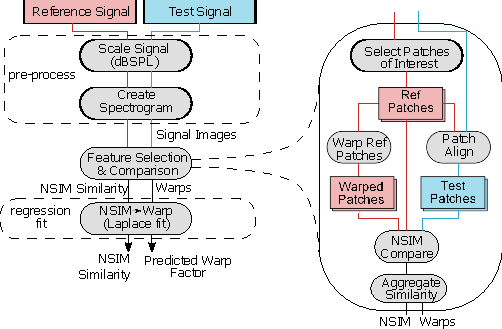
\includegraphics[width = .7\textwidth]{pic/visqol.pdf}
    \caption{Blokové schéma algoritmu ViSQOL\cite{article:visqol}}
    \label{pic:visqol}
\end{figure}

V první části označené jako předzpracování dochází k úrovňovému vyrovnání testovaného a referenčního signálu. Poté jsou pomocí Fourierovy krátkodobé transformace STFT oba signály převedeny na spektrogramy o třiceti frekvenčních pásmech logaritmicky rozdělených od 250 Hz do 8 kHz.

Část označená jako \textit{Feature Selection \& Comparsion} slouží k identifikaci vzájemně korespondujících políček\footnote{Anglicky označována jako \textit{patches}. Žádný dosavadní český překlad nebyl nalezen a z možností ve slovníku slovo políčko nejlépe významově koresponduje.}. Rozměr políčka je 30 rámců x 30 frekvenčních pásem. Algoritmus z obou zpracovávaných signálů vybírá tři takováto políčka nalezením maxima v pásmech 2, 6 a 10, se středními frekvencemi zhruba 250 Hz, 450 Hz a 750 Hz.
Poté je na korespondující políčka aplikována metoda výpočtu rozdílu pomocí kvadratické střední chyby\footnote{RMSE (Root Mean Squared Error)} rámec po rámci a pomocí minima této hodnoty jsou políčka zarovnána.

V posledním kroku se na políčka aplikuje NSIM, který vypočítá rozdílové skóre od nuly do jedné, kde nulové hodnocení dostávají signály bez jakékoli podobnosti a jedničku signály identické. Zároveň algoritmus vrací míru časového zkreslení (\textit{Time Warping}).

\section{Metody v multimediální technice}
\subsection{PEAQ}

\textit{Perceived Evaluation of Audio Quality} zkráceně PEAQ je objektivní metoda hodnocení vnímané kvality zvuku popsaná v ITU-R BS.1387-1 \cite{itur:1387}. Princip metody je zobrazen na obrázku \ref{pic:peaq}. Jedná se o intruzivní metodu, které je třeba dodat společně se zkresleným signálem signál referenční. Ty jsou převedeny do frekvenční oblasti. Jejich spektrální reprezentace prochází modelem slyšení a následně jsou z nich spočítány \textit{Model Output Values} zkráceně $MOV$. V závěru jsou v bloku zvaném \textit{Artificial Neural Network} provedeny výpočty simulující kognitivní procesy mozku. Výsledkem algoritmu je parametr zvaný $ODG$ (\textit{Objective Differemce Grade}), což je ekvivalent jednotky $SDG$, představené v podkapitole \ref{subchapter:impairment}

\begin{figure}[h]
    \centering
    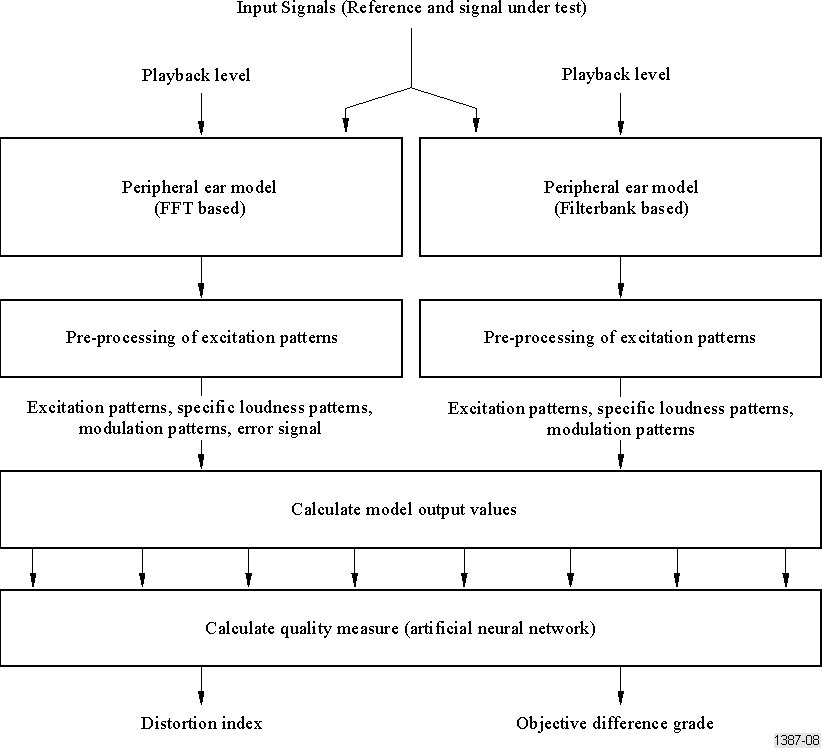
\includegraphics[width = .75\textwidth]{pic/peaq2.pdf}
    \caption{Blokové schéma algoritmu PEAQ}
    \label{pic:peaq}
\end{figure}

Model PEAQ existuje ve dvou verzích. Základní (\textit{Basic}) a pokročilé (\textit{Advanced}). Ta se od první liší především mírou komplexity výpočtů v sluchové a kognitivní části a použitím druhého modelu sluchové cesty založené na bance filtrů.

\begin{table}[h]
\centering
\begin{tabular}{|c|c|c|}
\hline
Název MOV & Model & Popis \\ \hline
\multicolumn{3}{|c|}{PEAQ Basic} \\ \hline
$BandwidthRef_B$ & FFT & Šířka pásma referenčního signálu \\ \hline
$BandwidthTest_B$ & FFT & Šířka pásma testovaného signálu \\ \hline
$Total NMR_B$ & FFT & Poměr Šum/Maska \\ \hline
$WinModDiff1_B$ & FFT & Váhovaný modulační rozdíl \\ \hline
$ADB_B$ & FFT & Průměrné blokové zkreslení \\ \hline
$EHS_B$ & FFT & Harmonická struktura chyb \\ \hline
$AvgModDiff1_B$ & FFT & Průměrný modulační rozdíl 1 \\ \hline
$AvgModDiff2_B$ & FFT & Průměrný modulační rozdíl 2 \\ \hline
$RmsNoiseLoud_B$ & FFT & Hlasitost zkreslení \\ \hline
$MFPD_B$ & FFT & Maximální vážená pravděpodobnost detekce \\ \hline
$RelDistFrames_B$ & FFT & Vzájemně zkreslené rámce \\ \hline
\multicolumn{3}{|c|}{PEAQ Advanced} \\ \hline
$RmsModDiff_A$ & Banka Filtrů &  \\ \hline
$RmsNoiseLoudAsym_A$ & Banka Filtrů & Hlasitost zkreslení \\ \hline
$Segmental NMR_B$ & FFT & Poměr Šum/Maska \\ \hline
$EHS_B$ & FFT & Harmonická struktura chyb \\ \hline
$AvgLinDist_A$ & Banka Filtrů & Lineární zkreslení \\ \hline
\end{tabular}
\caption{Seznam parametrů MOV}
\label{table:movs}
\end{table}

Algoritmus PEAQ předpokládá, že signály jsou vzorkovány kmitočtem 48 kHz a zároveň jsou časově a úrovňově vyrovnané. Po načtení je rozdělí do rámců o 2048 vzorcích s vzájemným 50\% překryvem. Dále je na rámce aplikováno Hannovo okno a pomocí diskrétní Fourierovy transformace jsou převedeny do frekvenční domény.

Model sluchové cesty se skládá z různých filtrů, reprezentace vnitřního šumu a výpočtu rozprostírání frekvenčních složek pomocí násobení bankou tzv \textit{Spreading functions}. Výstupem těchto matematických operací jsou $MOV$, jejichž seznam je v tabulce \ref{table:movs}.

Neuronová síť je rovnice \ref{equation:peaq}, do které vstupují parametry $MOV$ a jejím výstupem je parametr $D_I$ (\textit{Distortion Index}), který je přepočítán na $ODG$.


\begin{equation}
    D_I = w_{yb} + \sum\limits_{p=0}^{P-1}{\big(w_y[p]\text{sig}(w_{wb}[p]+\sum\limits_{q=0}^{Q-1} w_x[q,p]M'_v[q])\big)}
    \label{equation:peaq}
\end{equation}

\noindent kde $w_{y}$, $w_{wb}$, $w_{x}$ jsou váhovací  koeficienty dostupné v \cite{kabal}, $Q$ je počet \textit{Model Output Values} značených $M'$ a $P$ je počet uzlů v takzvané \uv{skryté vrstvě} což je vnitřek orientovaného grafu popisujícího neuronovou síť. Základní model má uzly tři, v pokročilém je jich pět.   

Doporučení \cite{itur:1387} klade velmi striktní nároky na implementaci tohoto algoritmu. Definuje šestnáct párů hudebních vzorků, u jejichž hodnocení implementací algoritmu by se $D_I$ neměl lišit o $\pm$ 0.02\% od hodnot určených doporučením. Jednou z takových implementací je například program Opera od společnosti Opticom \cite{web:opticom}. 



\subsection{PEMO-Q}

V roce 2006 Rainer Hubner a Birger Kollmeier publikovali článek s názvem \textit{PEMO-Q - A New Method for Objective Audio Quality Assessment Using a Model of Audiotory Perception} \cite{article:pemoq}. V tom vysvětlují, že PEMO-Q vychází z algoritmu PEAQ. Rozšiřuje ale jeho přístup o hledání obecných artefaktů jakým je například \textit{pre-echo}\footnote{Zvuk vzniklý kompresí, který se ozývá dříve, než v původní nahrávce.}. Dále se pyšní použitím lepšího sluchového modelu, představeného v publikaci \cite{book:dau}, který byl v rámci testování a optimalizace porovnáván s daty z šesti velkých subjektivních testů, které provedla ITU a MPEG v letech 1990 až 1995. Blokové schéma tohoto modelu je na obrázku \ref{pic:pemoq}. Funkce celého algoritmu poté na obrázku \ref{pic:pemoq2}.

\begin{figure}[h]
    \centering
    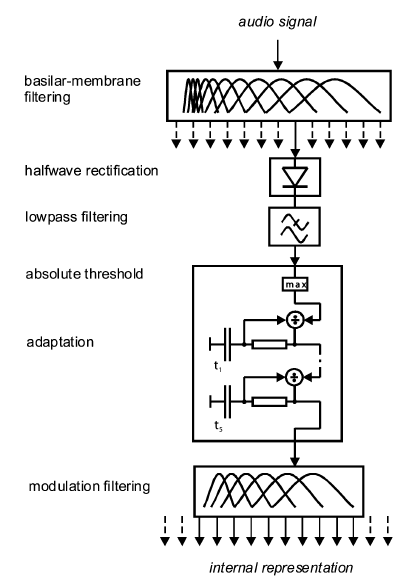
\includegraphics[width = .47\textwidth]{pic/pemoq.png}
    \caption{Blokové schéma modelu sluchové cesty v PEMO-Q\cite{article:pemoq}}
    \label{pic:pemoq}
\end{figure}

Prvním blokem je banka třiceti pěti gammatónových filtrů simulující funkci bazilární membrány. Střední kmitočty jednotlivých filtrů jsou v rozsahu od 235 Hz až po 14,5 kHz. Každá větev je zpracovávána nezávisle. Následné usměrnění a filtrace dolní propustí reprezentuje převod zvuku na nervové impulzy. Zpracovaný signál je přiveden do bloku adaptivní filtrace složeného z pěti zpětnovazebních smyček zapojených do kaskády. Na konci cesty je další banka osmi filtrů modelujících schopnost rozpoznání amplitudově modulovaného zvuku.

\begin{figure}[h]
    \centering
    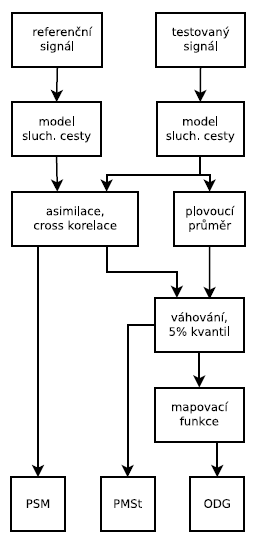
\includegraphics[width = .25\textwidth]{pic/pemoq2.png}
    \caption{Blokové schéma algoritmu PEMO-Q \cite{thesis:zalabak}}
    \label{pic:pemoq2}
\end{figure}

Před kognitivním zpracováním je provedena asimilace signálu. Jedná se o matematický průměr vnitřních tří-dimenzoinálních reprezentací (frekvenční, časové a modulační) testovaného a referenčního signálu tam, kde testovaný nabývá nižších hodnot než signál referenční. Tato operace vychází z poznatku, že \uv{chybějící} prvky jsou méně rušivé než prvky \uv{přidané}. 
Poté je provedena korelace pro každý modulační kanál zvlášť přes všechny časové a frekvenční hodnoty. Z kvadrátů výsledků korelačních funkcí je poté vypočítána hodnota $PSM$ (\textit{Perceptual Similarity Measure}) a z ní i hodnota $ODG$.

\subsection{ViSQOLAudio}

Evolucí původního algoritmu ViSQOL přestaveného v podkapitole \ref{subchapter:visqol} určeného k hodnocení hudebních signálů je tak zvaný ViSQOLAudio. V článku \textit{ViSQOLAudio: An objective audio quality metric for low bitrate codecs} \cite{article:visqolaudio} autoři tvrdí, že k adaptaci původní metody na hodnocení hudebních nahrávek bylo třeba jen drobných změn.

\medskip

Zde je jejich výčet:

\begin{itemize}
    \item Systém porovnávání políček referenčního a testovaného signálu je zachován, nicméně všechna políčka jsou nyní označena za \uv{aktivní} na rozdíl od původních třech signifikantních pro řečové signály.
    \item Množství frekvenčních pásem při předzpracování bylo rozšířeno na celé slyšitelné pásmo od 50 Hz do 20 kHz.
\end{itemize}